\documentclass[dvipsnames] {beamer}
\usepackage{cmlgc}
\usepackage{comment}
\usepackage{tikz}
\usefonttheme{serif}     % Font theme: serif
\usepackage[T2A]{fontenc}
\usepackage[utf8]{inputenc}
\usepackage[english,russian]{babel}
\usepackage{amssymb,amsfonts,amsmath,mathtext,cite,enumerate,float} %подключаем нужные пакеты расширений
% \usepackage{cyrillic}
\usepackage{color, colortbl}
\usepackage{multirow}
\usepackage{graphicx}
\usepackage{graphics}
\usepackage{multirow}
\usepackage{url}
\usepackage{hyperref}
\usepackage{animate}
\usepackage{pifont}
\usepackage{wasysym}
\usepackage{marvosym}
\usepackage{appendixnumberbeamer} 
\usepackage{pgfpages}
\usepackage{systeme,mathtools}
\usepackage{mathtools}
\usepackage{listings}
\usepackage{xcolor} % for setting colors


\usepackage{ragged2e} %выравнивание текста по ширине слайда (\justifying)
%\setbeamercolor{background canvas}{bg=violet}

\usetheme{Madrid}
%\usecolortheme{crane}

%=================================================

    \defbeamertemplate*{footline}{mytheme}{%
      \leavevmode%
      \hbox{%
      \begin{beamercolorbox}[wd=.2\paperwidth,ht=3ex,dp=1ex,center]{author in head/foot}%
        \usebeamerfont{author in head/foot}\insertshortauthor
      \end{beamercolorbox}%
      \begin{beamercolorbox}[wd=.7\paperwidth,ht=3ex,dp=1ex,center]{title in head/foot}%
        \usebeamerfont{title in head/foot}\insertshorttitle
      \end{beamercolorbox}%
      \begin{beamercolorbox}[wd=.1\paperwidth,ht=3ex,dp=1ex,right]{date in head/foot}%
        %\usebeamerfont{date in head/foot}\insertshortdate{}\hspace*{2em}
        %\insertframenumber{} / \inserttotalframenumber\hspace*{2ex} %номер текущего слайда / общее число слайдов
        \insertframenumber{} \hspace*{5ex}  %номер текущего слайда
      \end{beamercolorbox}}%
      \vskip0pt%
    }
    \usebeamertemplate{mytheme}
\beamertemplatenavigationsymbolsempty

\defbeamertemplate*{frametitle}{boldTitle}{%
    \begin{beamercolorbox}[wd=\paperwidth,ht=3ex,dp=3pt,center]{title in head/foot}%
%        \ \textit{\textbf{\insertframetitle}} % курсивный заголовок слайда 
        \ \textbf{\insertframetitle}
    \end{beamercolorbox}
}
\usebeamertemplate{boldTitle}
\setbeamercovered{dynamic}

\setbeameroption{hide notes} % Only slides
%\setbeameroption{show only notes} % Only notes
%\setbeameroption{show notes on second screen=right} % Both
%\setbeamertemplate{note page}[plain]


%=================================================
% \titlegraphic{
\includegraphics[width=\textwidth]{logo_conf.png}}
\addtobeamertemplate{title page}{\centering 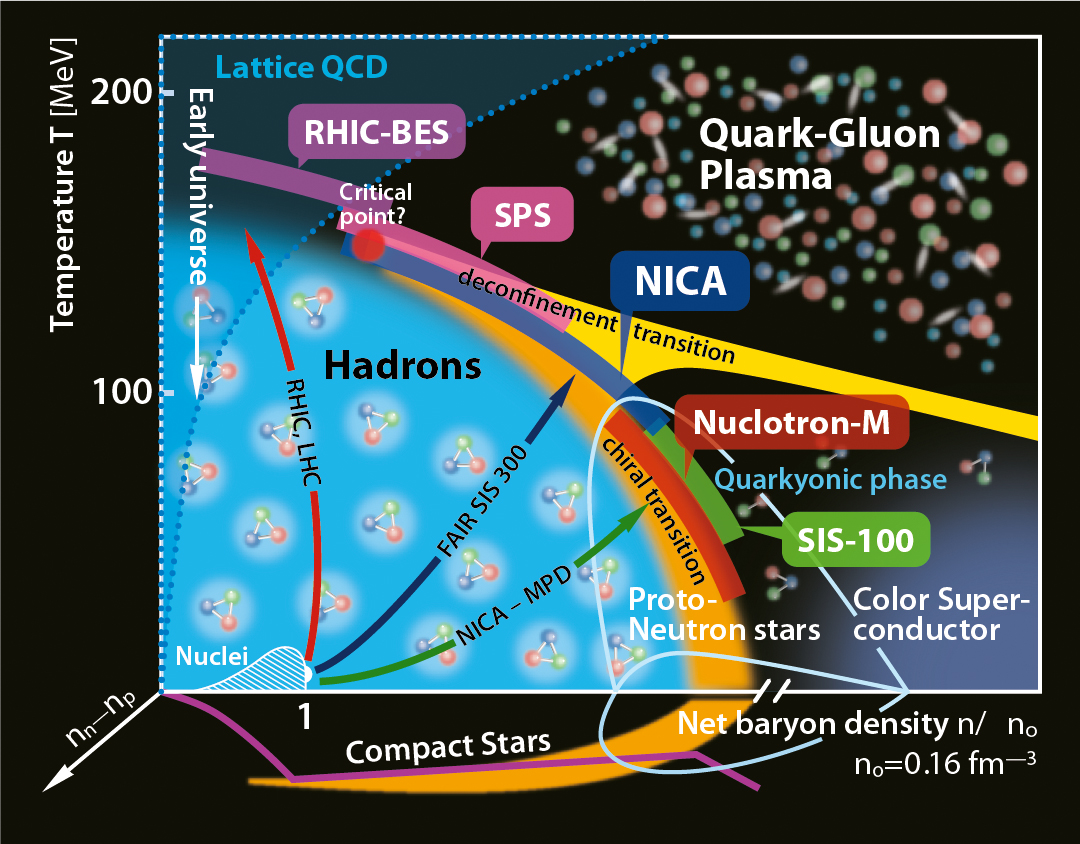
\includegraphics[scale=0.1]{Phase_diagram.jpg}}{}
\title[\bf Dubna, CSQCD 2017]{\textbf{\large {Simulation of NICA/MPD with THESEUS as an attempt to investigate effects of a QCD phase transition in the EoS on HIC observables}}}

%\author[P.~Batyuk]{\textit{\textbf{{\footnotesize \underline{P.~Batyuk}, L.~Malinina (SINP MSU, JINR), \\ O.~Rogachevskiy (JINR)}}} \\
%  on behalf of the MPD collaboration}
\author[\bf P.~Batyuk]{\textit{\textbf{{\footnotesize \underline{P.~Batyuk}}}} \\
 on behalf of the MPD collaboration} 
\institute{\url{pavel.batyuk@jinr.ru}  \\ VBLHEP, JINR}

 \date{{\textbf{September 28, 2017}}}  
% \newpage \footnotesize April 14, 2016}}
  
\lstset{
%    frame=tb, % draw a frame at the top and bottom of the code block
    tabsize=4, % tab space width
    showstringspaces=false, % don't mark spaces in strings
 %   numbers=left, % display line numbers on the left
    commentstyle=\color{blue}, % comment color
    keywordstyle=\color{blue}, % keyword color
    stringstyle=\color{red} % string color
}

    
\begin{document}
\maketitle

\begin{frame}
  \frametitle{Outline:}
  \bf
  \begin{itemize}
  \item Three-fluid Hydrodynamics-based Event Simulator Extended by UrQMD final State interactions (THESEUS) 
  \item NICA Complex, NICA/MPD, MPDROOT ...
  \item First results on baryon stopping power and direct flow as a result of MC simulation of NICA/MPD
  \end{itemize}
\end{frame}

\begin{frame}
  \frametitle{{\tiny Three-fluid Hydrodynamics-based Event Simulator Extended by UrQMD final State interaction}}
  \begin{columns}[c]
    \column{.49\textwidth}
    \begin{block}{}
    \begin{figure}[H]
      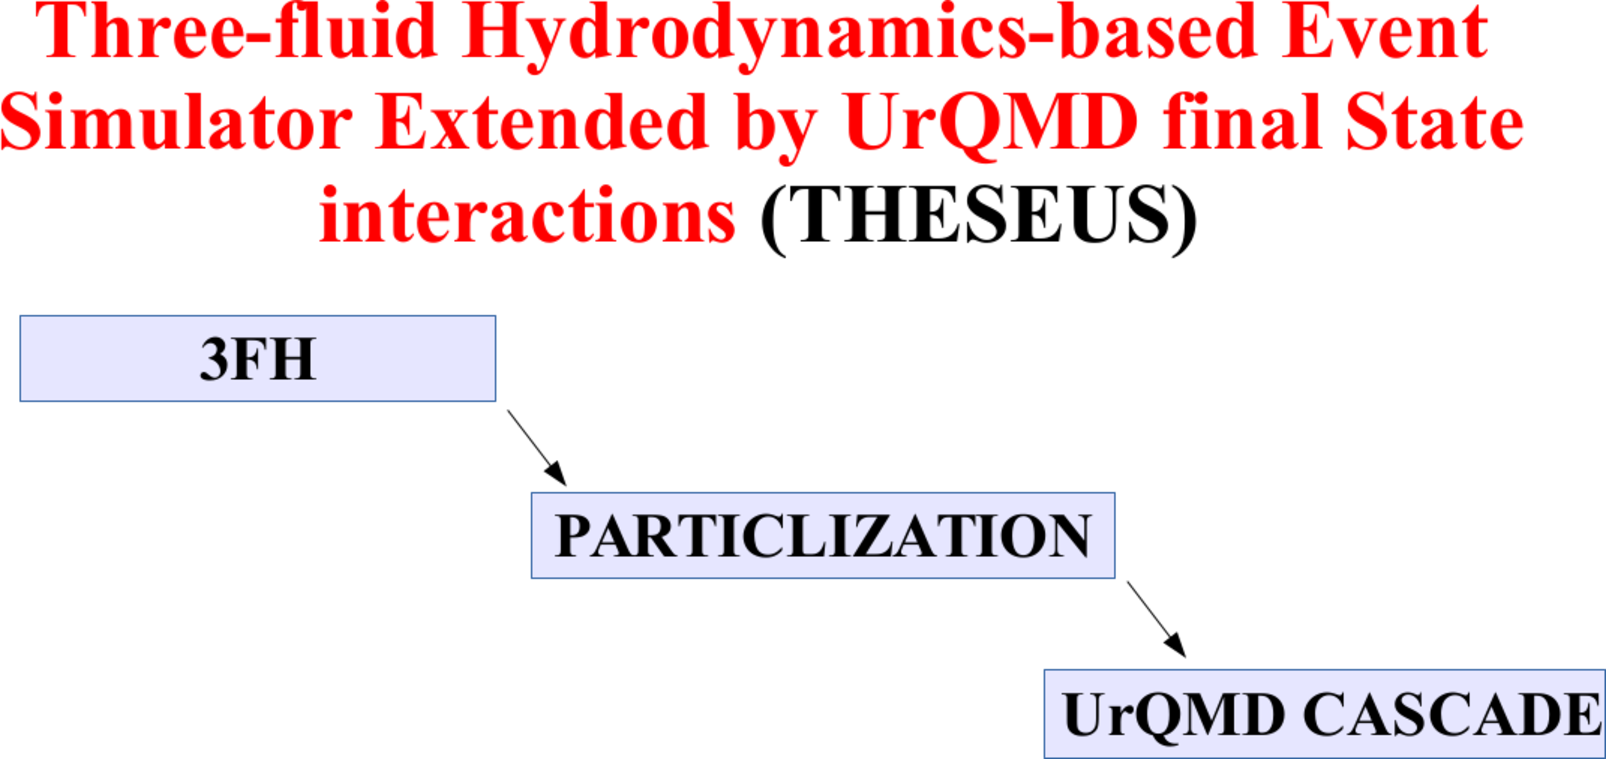
\includegraphics[width=1.\textwidth]{THESEUS_model_cut.pdf}
    \end{figure}
    \end{block}
    \column{.49\textwidth}
    \begin{block}{}
     {\small \bf 
      \begin{itemize}      
      \item The simulation was performed with the crossover EoS without freeze-out.
      \item Very high baryon densities are reached in the central region of the colliding system.
      \end{itemize}
      }
    \end{block}
  \end{columns}
  

  \begin{block}{\bf \centering 3FH-model (see report of Yu. B. Ivanov, CSQCD-VI):}
  \begin{figure}[H]
    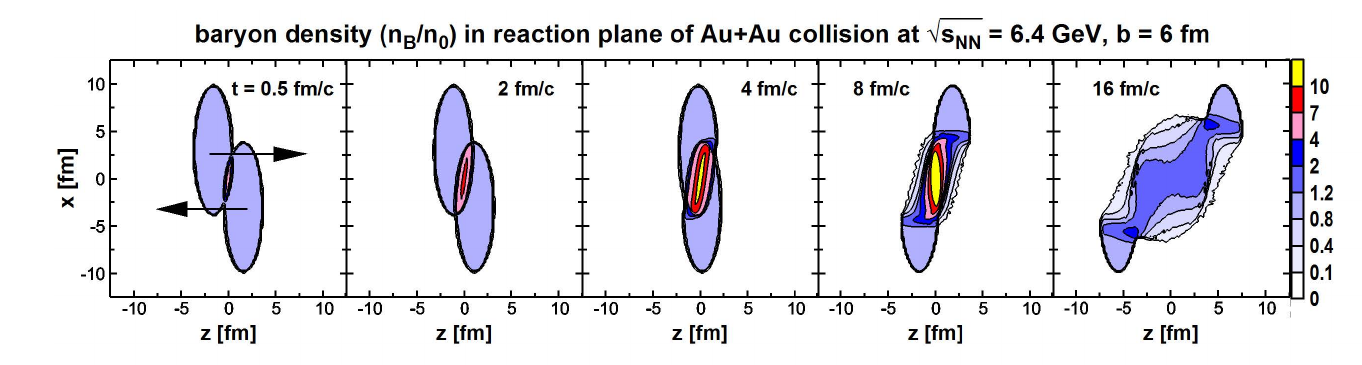
\includegraphics[width=1.\textwidth]{baryon_density.jpg}
  \end{figure}
  \end{block}
\end{frame}

\begin{frame}
  \frametitle{Test of the particlization and cascade routines}
  \begin{columns}[c]
    \column{.68\textwidth}
    \begin{block}{\bf \centering $p_{T}$-spectra:}
    \begin{figure}[H]
      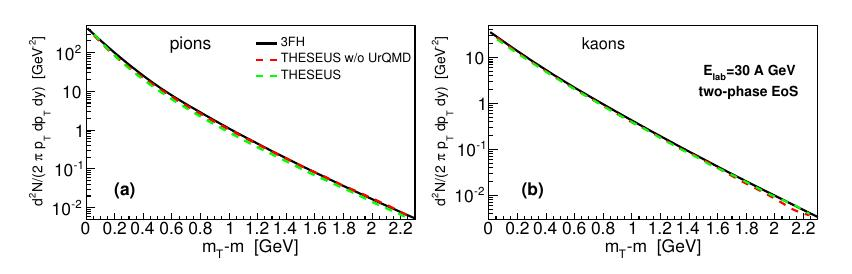
\includegraphics[width=1.\textwidth]{pT_spectra.jpg}
    \end{figure}
  \end{block}
  
  \begin{block}{\bf \centering Rapidity distribution:}
   \begin{figure}[H]
     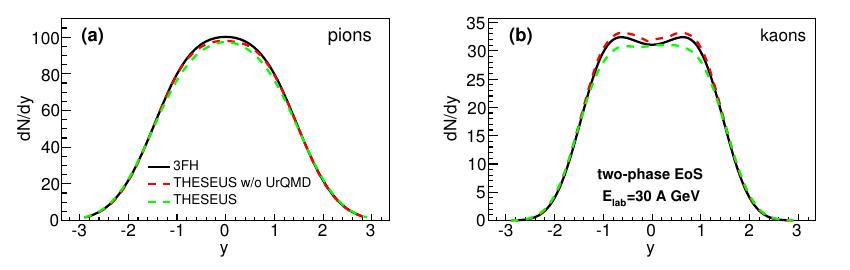
\includegraphics[width=1.\textwidth]{ySpectra.jpg}
   \end{figure}
  \end{block}
  \column{.29\textwidth}
  \begin{block}{}
    \begin{center}
      {\small \bf AuAu @ 30~AGeV, b = 2fm, 2-phase EoS}
  \end{center}
  \end{block}
  
  \begin{block}{\bf \centering UrQMD hadronic rescattering:}
    {\footnotesize \bf
    \begin{itemize}
    \item leads to a slight steepening of the pion $p_{T}$-spectrum.
    \item smeares the double-peak structure in the kaon rapidity spectrum.
    \end{itemize}
    }
  \end{block}
  \end{columns}
\end{frame}


\begin{frame}[shrink=40]
  \bf
  \frametitle{NICA Complex}
  \begin{columns}[c]
    \column{.40\textwidth}
    \begin{block}{\centering \bf General characteristics:}
      \centering  Beams - {\color{red}$p$, $d$ ... $^{197}Au^{79+}$} \\
      \centering  Collision energy: 
      \begin{columns}[c]
        \column{.49\textwidth}
        $\sqrt{s_{NN}}$ = {\color{red} 4 - 11} GeV
        \column{.49\textwidth}
        $E_{lab}$ =  {\color{red}1 - 6} AGeV
      \end{columns}
      Luminosity: {\color{red}$10^{27}~cm^{-2}s^{-1}$} (Au), {\color{red}$10^{32}$} (p)

    \end{block}
    \column{.40\textwidth}
    \begin{block}{}
      \bf
      \centering
       See report of A. Sorin, CSQCD-VI (26.09.2017) 
    \end{block}
    \begin{block}{\centering \bf Experiments:}
      \begin{itemize}
      \item 2 interaction points - {\color{red}MPD} and  {\color{red}SPD}
      \item Fixed target experiment -  {\color{red}BM@N}
      \end{itemize}
    \end{block}
  \end{columns}
  \begin{columns}[c]
   % \column{.05\textwidth}
    \column{.75\textwidth}
    \begin{block}{}
      \begin{figure}[H]
        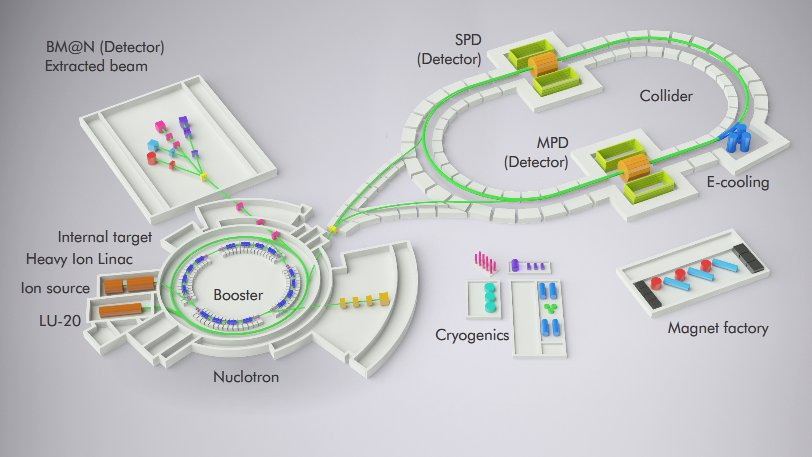
\includegraphics[width=1.\linewidth]{nica_complex1.png}
      \end{figure}
      % \centering The general contractor is  {\color{red} STRABAG} (Bodostal-3 \& PCJ are the sub-contactors)
    \end{block}
    \column{.20\textwidth}
    \begin{block}{}
    \begin{itemize}
    \item {\color{red} 2017:} extracted beams of heavy ions are available within the BM@N experiment
    \item {\color{red} 2019}: a first configuration of the MPD setup available.
    \item {\color{red} 2023}: commissioning of the fully designed NICA-complex is foreseen.	
    \end{itemize}
 \end{block}

  \end{columns}
\end{frame}

\begin{frame}[shrink=25]
  \bf
  \frametitle{\centering \bf {\small MultiPurpose Detector (MPD) for $A + A$ collisions @ NICA}}
  \begin{columns}[c]
    \column{.4\textwidth}
    \begin{block}{\bf \centering Layout:}
      \begin{figure}[H]
        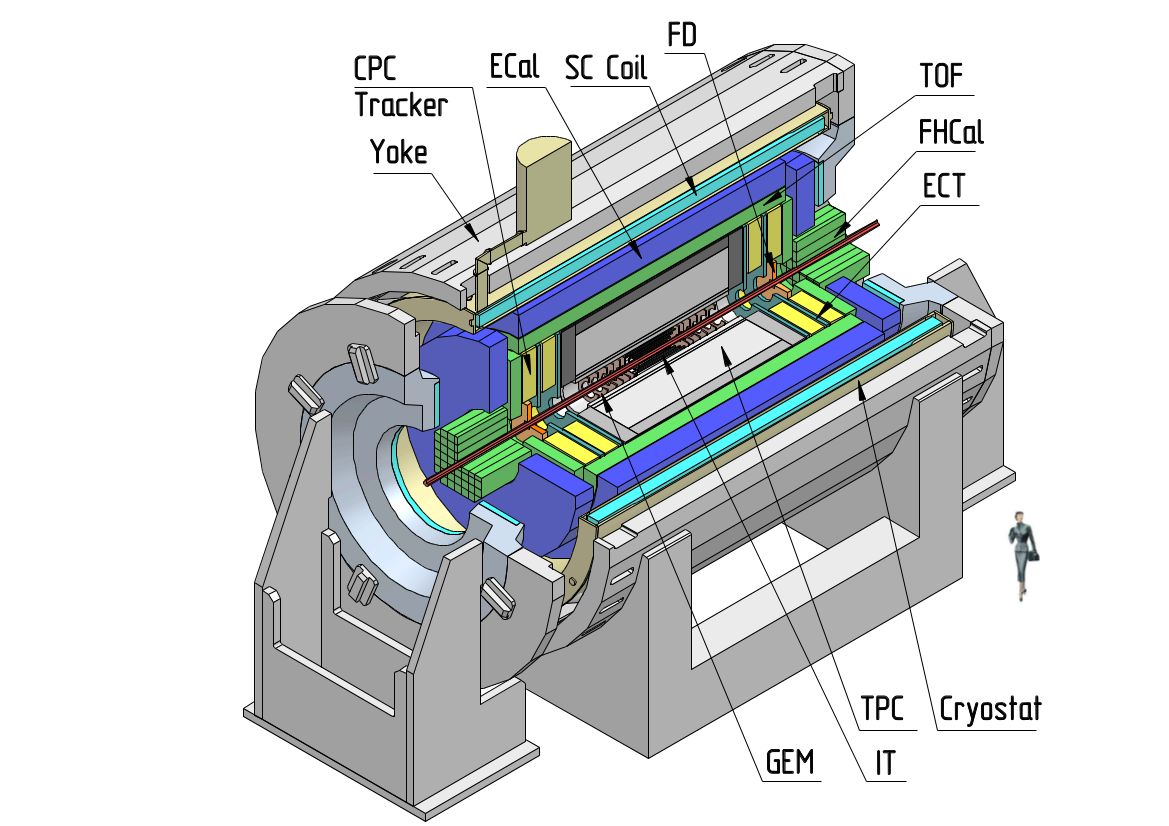
\includegraphics[width=.96\textwidth]{mpd.png}
      \end{figure}
    \end{block}
    \begin{block}{\bf \centering Momentum resolution:}
    \begin{figure}[H]
        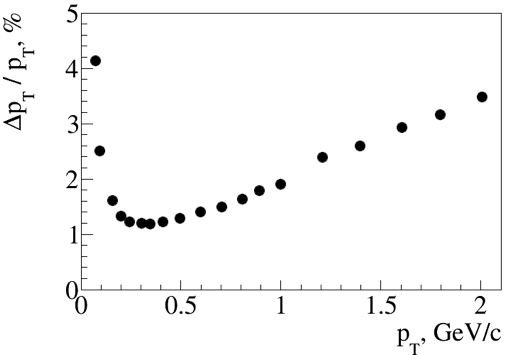
\includegraphics[width=.96\textwidth]{mom_res_mpd.png}
      \end{figure}    	
    \end{block}

    \column{.55\textwidth}
    \begin{block}{\bf \centering Benefits:}
      \begin{itemize}
      \item Hermeticity, $2\pi$-acceptance in azimuth
      \item 3D-tracking (TPC, ECT)
      \item Vertex high-resolution (IT)
      \item Powerful PID (TPC, TOF, ECAL)
        \begin{itemize}
        \item $\pi, K$ up to 1.5 GeV/c
        \item $K, p$ up to 3 GeV/c
        \item $\gamma, e$ from 0.1 GeV/c up to 3 GeV/c
        \end{itemize}
      \item Precise event characterization (FHCAL = ZDC) (centrality determination, reaction plane ...)
      \item Fast timing and triggering (FFD)
      \item Low material budget
      \item High event rate (up to 7 kHz) 
      \end{itemize}
    \end{block}
  \end{columns}
\end{frame}

 \begin{frame}[shrink=35]
  \bf
  \frametitle{\bf \centering Simulation Framework for MPD (MPDROOT)} 
  \begin{columns}[c]
    \column{.60\textwidth}
    \begin{block}{}
      \begin{figure}[H]
        
\includegraphics[width=1.\textwidth]{mpdroot_web.png}
      \end{figure}
    \end{block}
    \column{.30\textwidth}
    \begin{block}{\bf \centering MPDROOT home web-page:}
      http://mpd.jinr.ru
    \end{block}
  \end{columns}
  \begin{columns}[c]
    \column{.20\textwidth}
    \begin{block}{}
      \begin{itemize}
      \item News
      \item Software repositories
      \item Software tests
      \item Forums
      \item Database for physics run
      \item E.t.c.
      \end{itemize}
    \end{block}
    \column{.33\textwidth}
    \begin{block}{}
      \begin{figure}[H]
        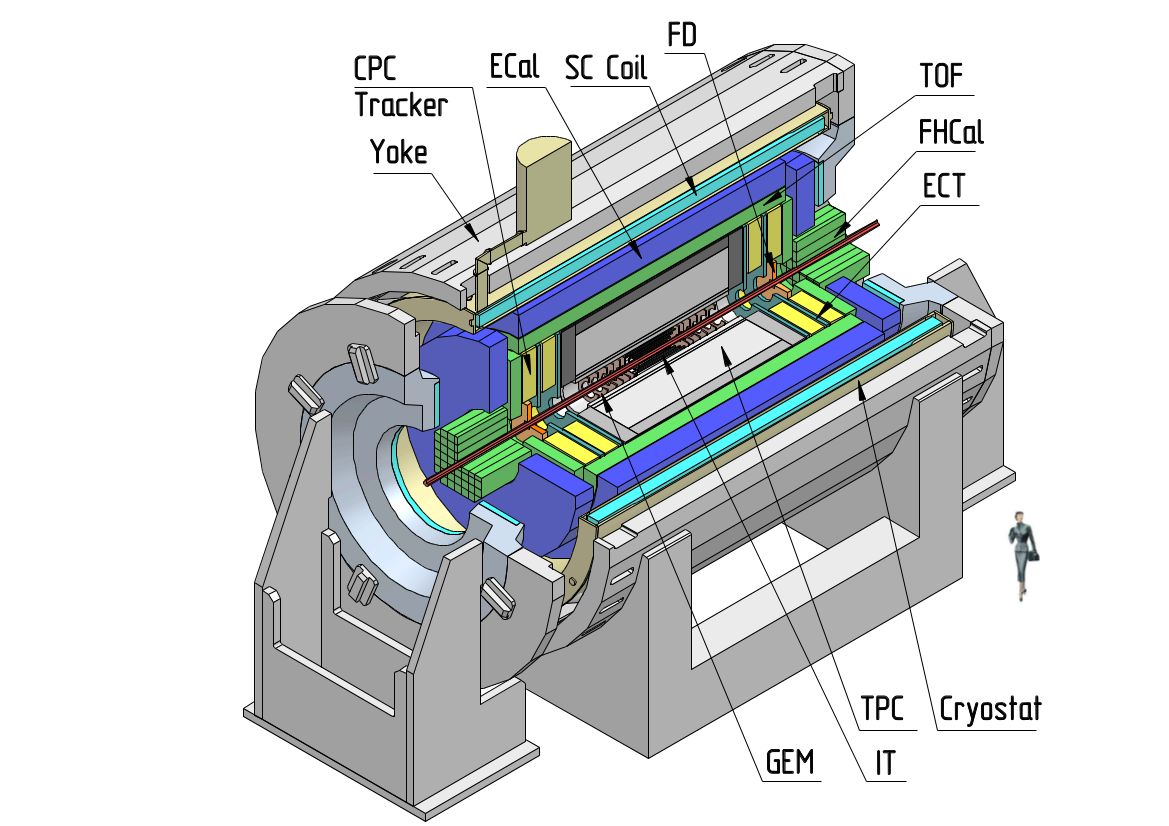
\includegraphics[width=1.\textwidth]{mpd.png}
      \end{figure}
    \end{block}
    \column{.40\textwidth}
    \begin{block}{\bf \centering Physics models available: }
      \begin{itemize}
      \item UrQMD / Hybrid UrQMD / vHLLE + UrQMD
      \item QGSM / LAGQSM
      \item HSD / PHSD
      \item {\Large {\color{red} THESEUS}}
      \end{itemize}
    \end{block}
  \end{columns}
  \begin{columns}[c]
  
    \column{.68\textwidth}
    \begin{block}{\bf \centering Benefits:}
      {\small 
      \begin{itemize}
      \item Inherits basic properties from FairRoot, C++ classes
      \item Extended set of event generators for heavy-ion collisions
      \item Detector composition and geometry; particle propagation by GEANT3/4
      \item Advanced detector response functions, realistic tracking and PID included
      \item Event display for Monte-Carlo and experimental data 
      \end{itemize}
      }
    \end{block}

    \column{.27\textwidth}
    \begin{block}{}
      \begin{center}
        {\Large \color{red} \bf All main macroses to be used for sim \& reco have been adopted for THESEUS input}
      \end{center}
    \end{block}
  \end{columns}
 \end{frame}

 \begin{frame}
   \frametitle{\bf \centering THESEUS: data sets available}
 \end{frame}


 
 \begin{frame}[shrink=5]
   \frametitle{Direct flow of protons(THESEUS)}
   \begin{columns}[c]
     \column{.1\textwidth}
     \column{.31\textwidth}
     \begin{block}{\bf \centering $\sqrt{s_{NN}}$ = 5.6 GeV}
        \begin{figure}[H]
      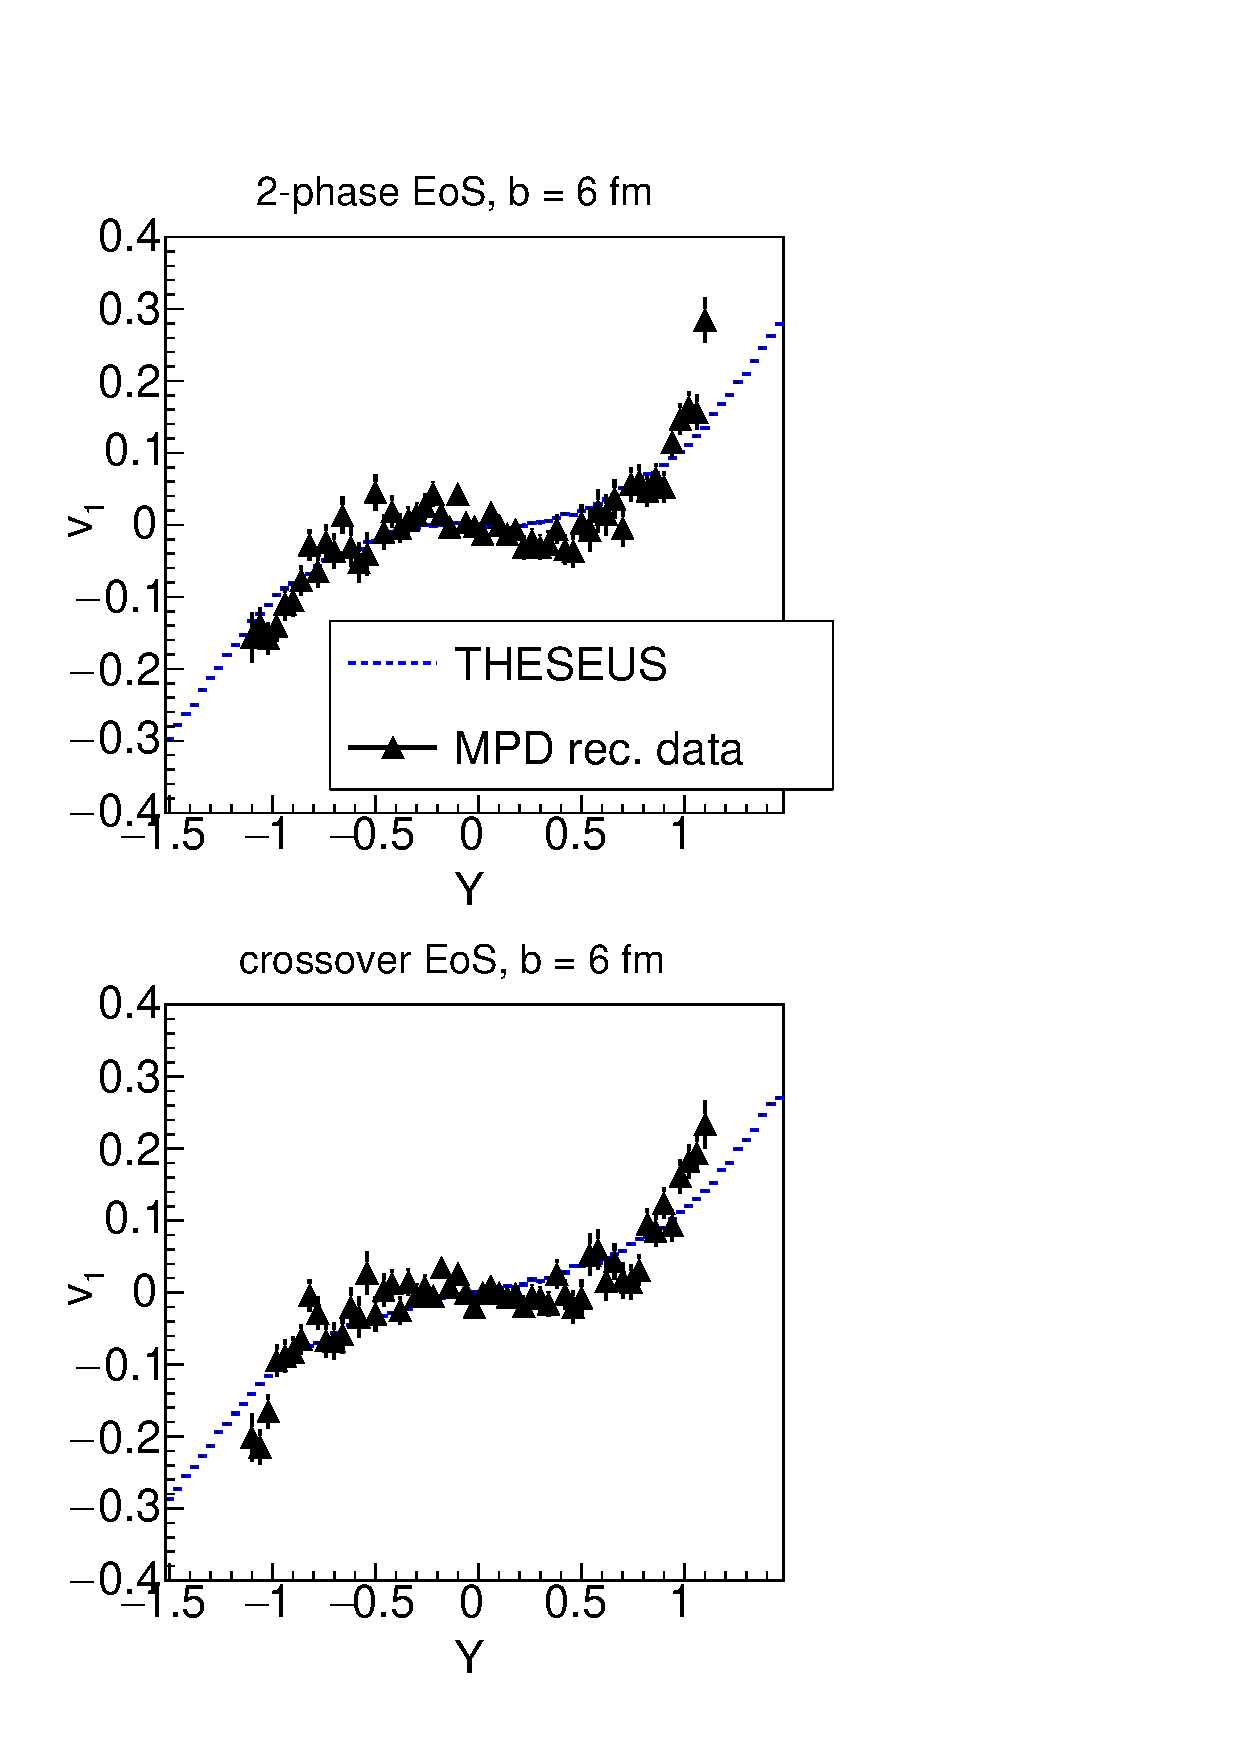
\includegraphics[width=1.\textwidth]{energy15AGeV_proton_urqON.pdf}
        \end{figure}
     \end{block}
     \column{.31\textwidth}
     \begin{block}{\bf \centering $\sqrt{s_{NN}}$ = 11.6 GeV}
        \begin{figure}[H]
      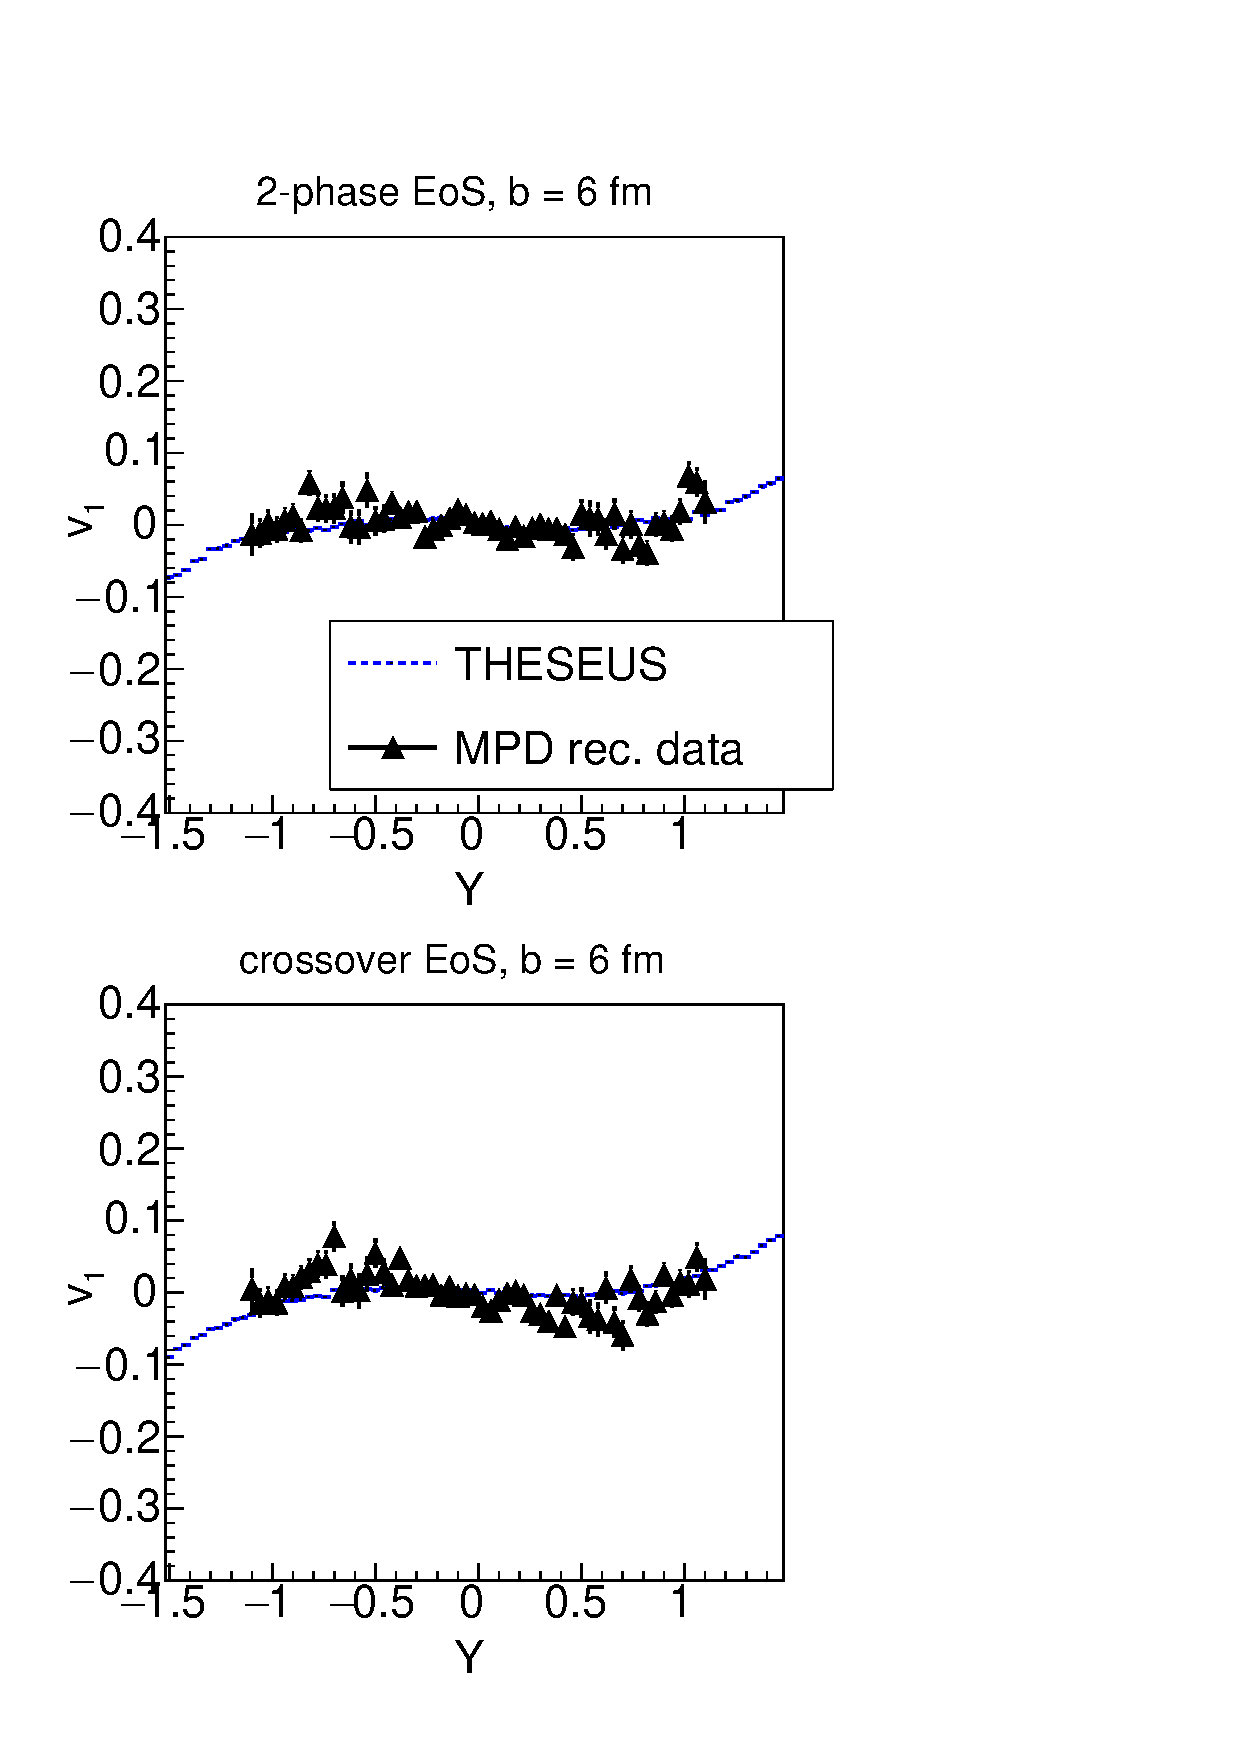
\includegraphics[width=1.\textwidth]{energy70AGeV_proton_urqON.pdf}
        \end{figure}     
     \end{block}
     \column{.1\textwidth}
    
   \end{columns}
 \end{frame}

\begin{frame}[shrink=5]
   \frametitle{Direct flow of protons(THESEUS w/o UrQMD)}
   \begin{columns}[c]
     \column{.31\textwidth}
     \begin{block}{\bf \centering $\sqrt{s_{NN}}$ = 5.6 GeV}
        \begin{figure}[H]
      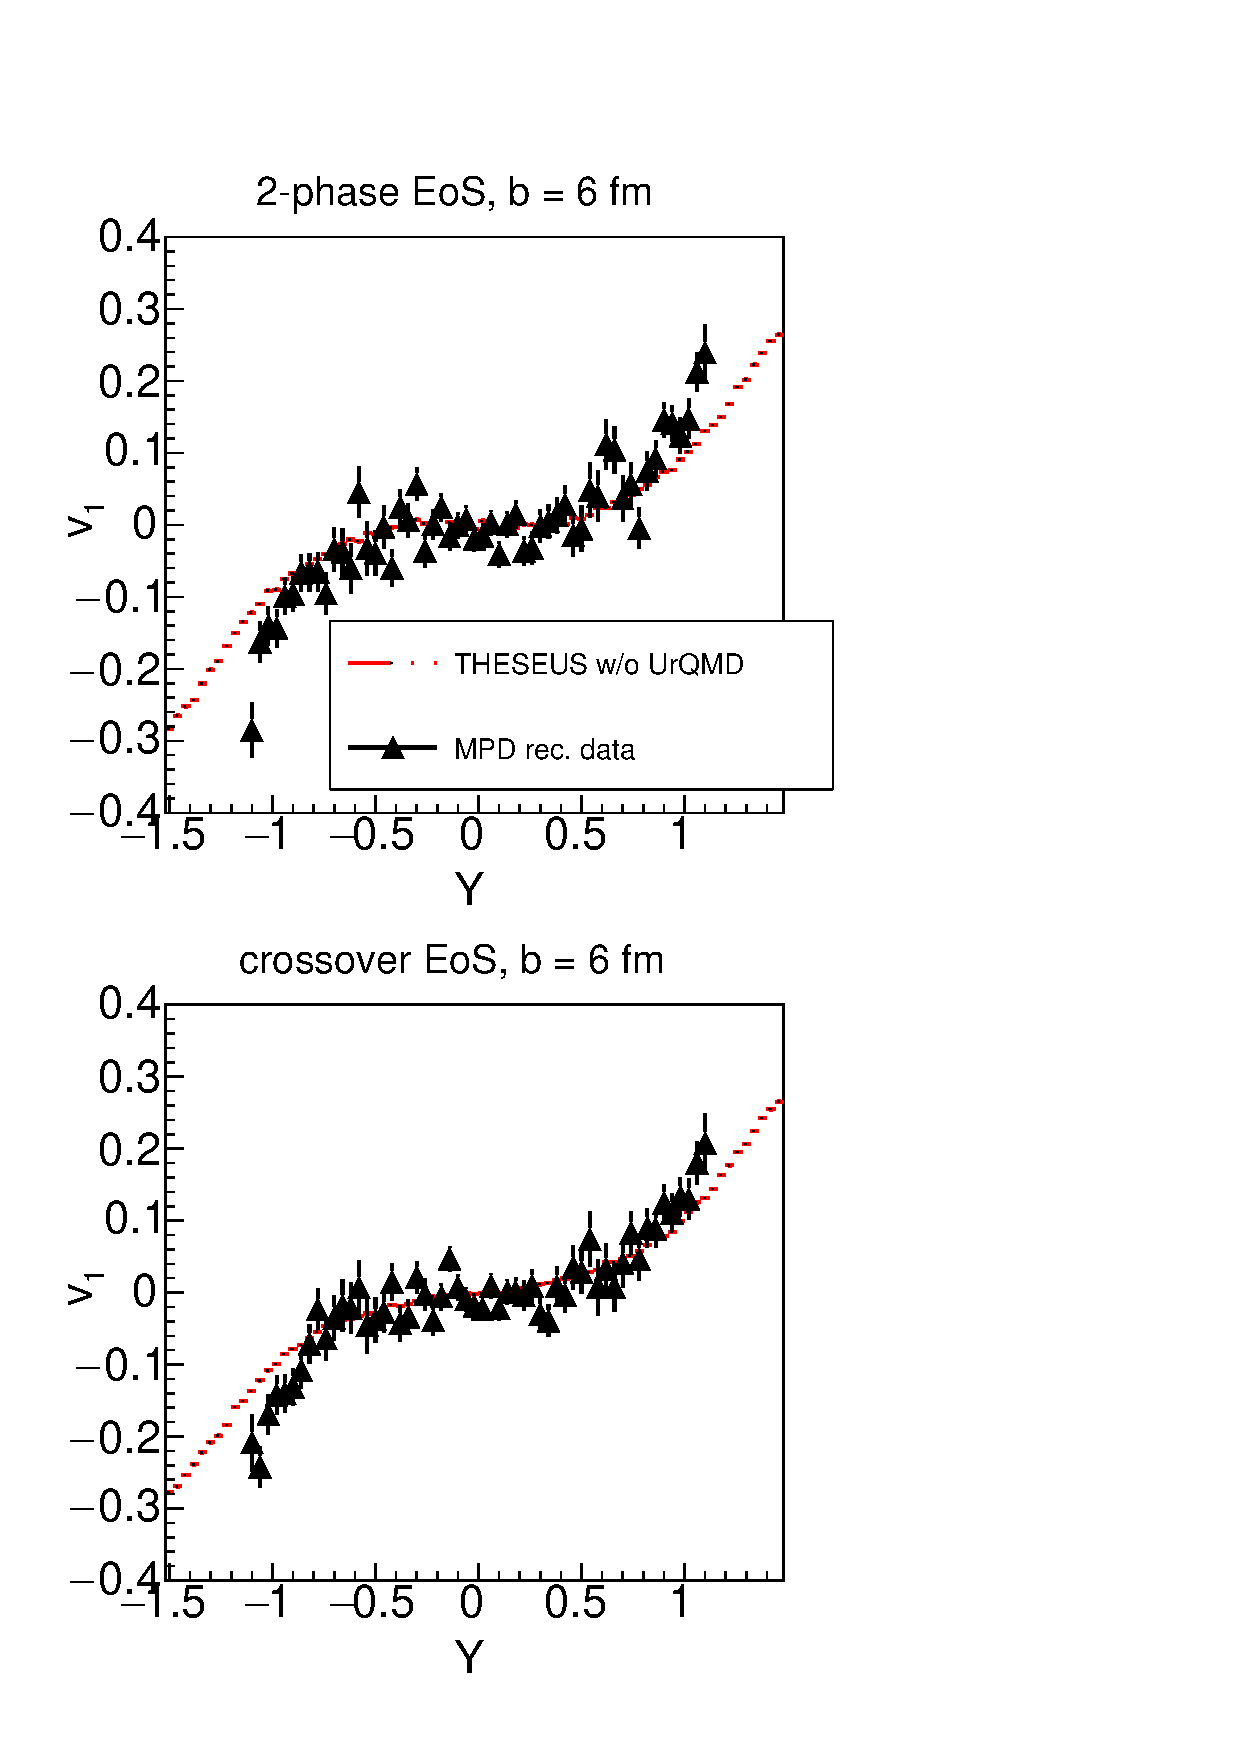
\includegraphics[width=1.\textwidth]{energy15AGeV_proton_urqOFF.pdf}
        \end{figure}
     \end{block}
     
     \column{.31\textwidth}
     \begin{block}{\bf \centering $\sqrt{s_{NN}}$ = 11.6 GeV}
        \begin{figure}[H]
      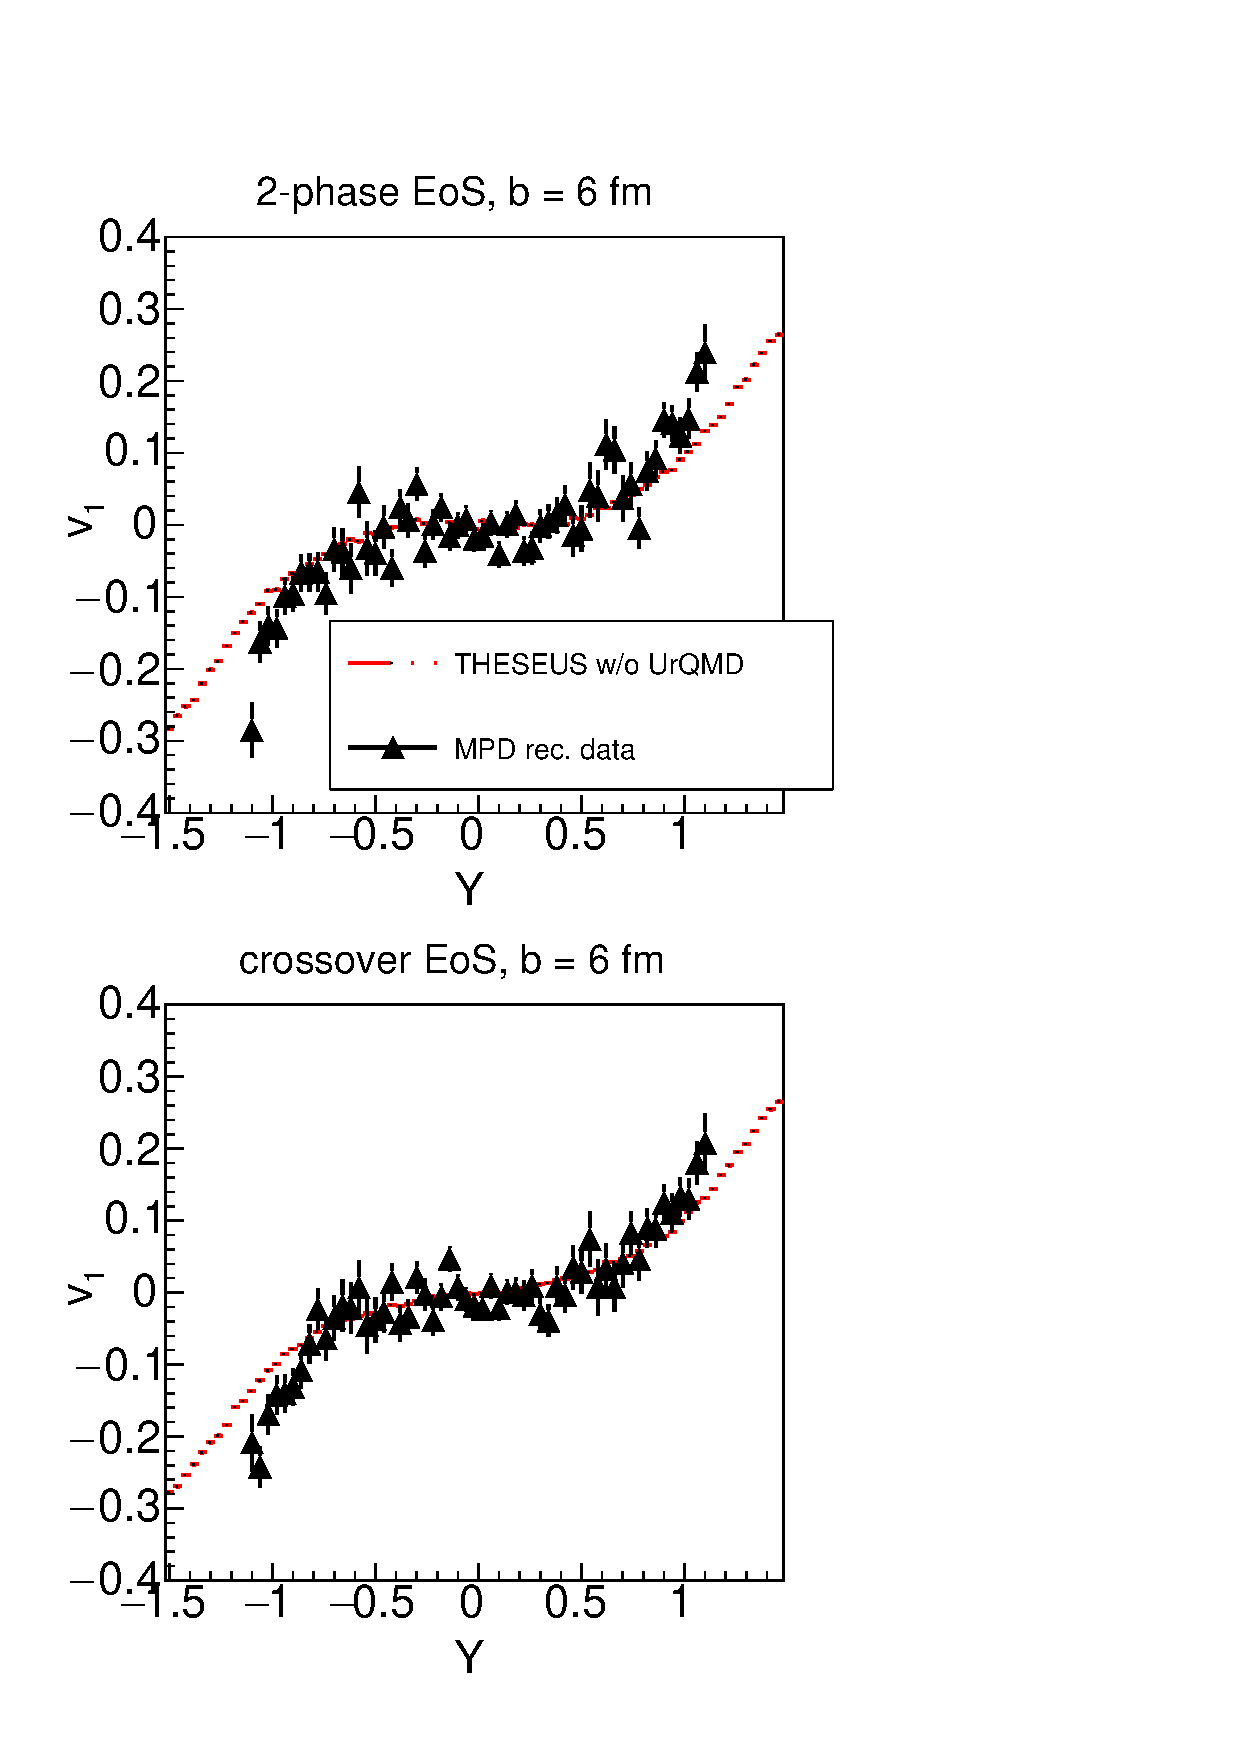
\includegraphics[width=1.\textwidth]{energy70AGeV_proton_urqOFF.pdf}
        \end{figure}     
     \end{block}
     
     \column{.33\textwidth}
     \begin{block}{}
       {\color {red} \bf Results on reconstructed flow are preliminary: statistics should be increased, amendments in reco. algorithm are also in progress}
     \end{block}
     \begin{block}{}
       \bf
          {\color {blue} Reco output coincides better in midrapidity region with model input when no UrQMD rescatterings are taken into account}  
     \end{block}
   \end{columns}
 \end{frame}

\begin{frame}[shrink=20]
  \frametitle{Direct flow of protons, $dv_{1} / dy$}
 % \begin{block}{}
  %  \bf Actual version of PID has been used. $P_{particle = proton} > 0.9$ 
  %\end{block}
  \begin{columns}[c]
    \column{.3\textwidth}
    \begin{block}{{\tiny \bf \centering THESEUS:}}
    \begin{figure}[H]
      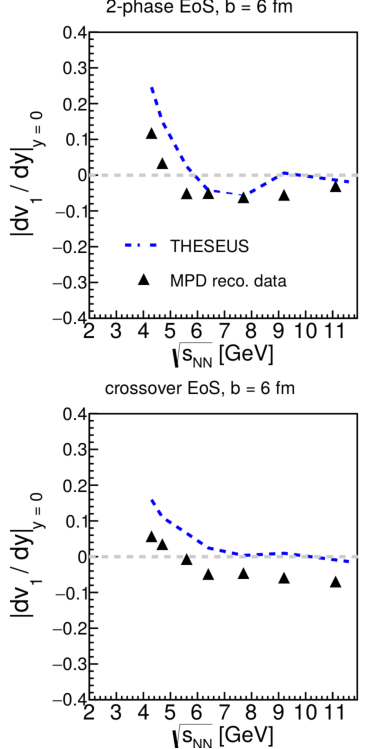
\includegraphics[width=.99\textwidth]{slopeProtons_6fm_urqON.pdf}
    \end{figure}
    \end{block}

    
    \column{.3\textwidth}
    \begin{block}{{\tiny \bf \centering THESEUS w/o UrQMD:}}
    \begin{figure}[H]
      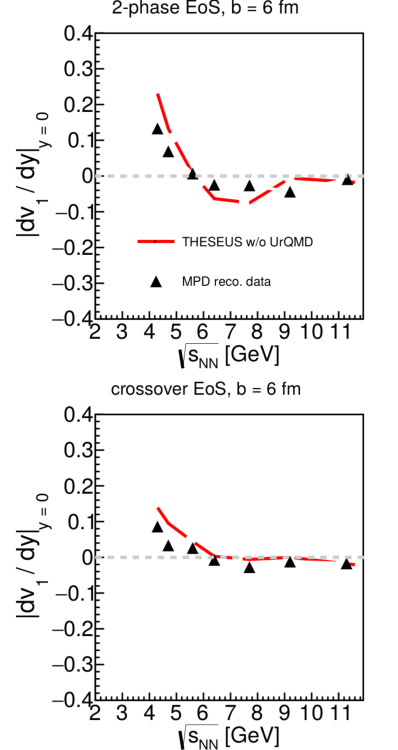
\includegraphics[width=1.01\textwidth]{slopeProtons_6fm_urqOFF.pdf}
    \end{figure}
    \end{block}

    
    \column{.3\textwidth}
    %\begin{block}{{\tiny \bf \centering Comparison with exp. data available:}}
      {\tiny \bf \centering Comparison with exp. data available:}
      \begin{block}{ \tiny \bf \centering Phys. Rev. C 94, 044917 (2016)}
      \begin{figure}[H]
        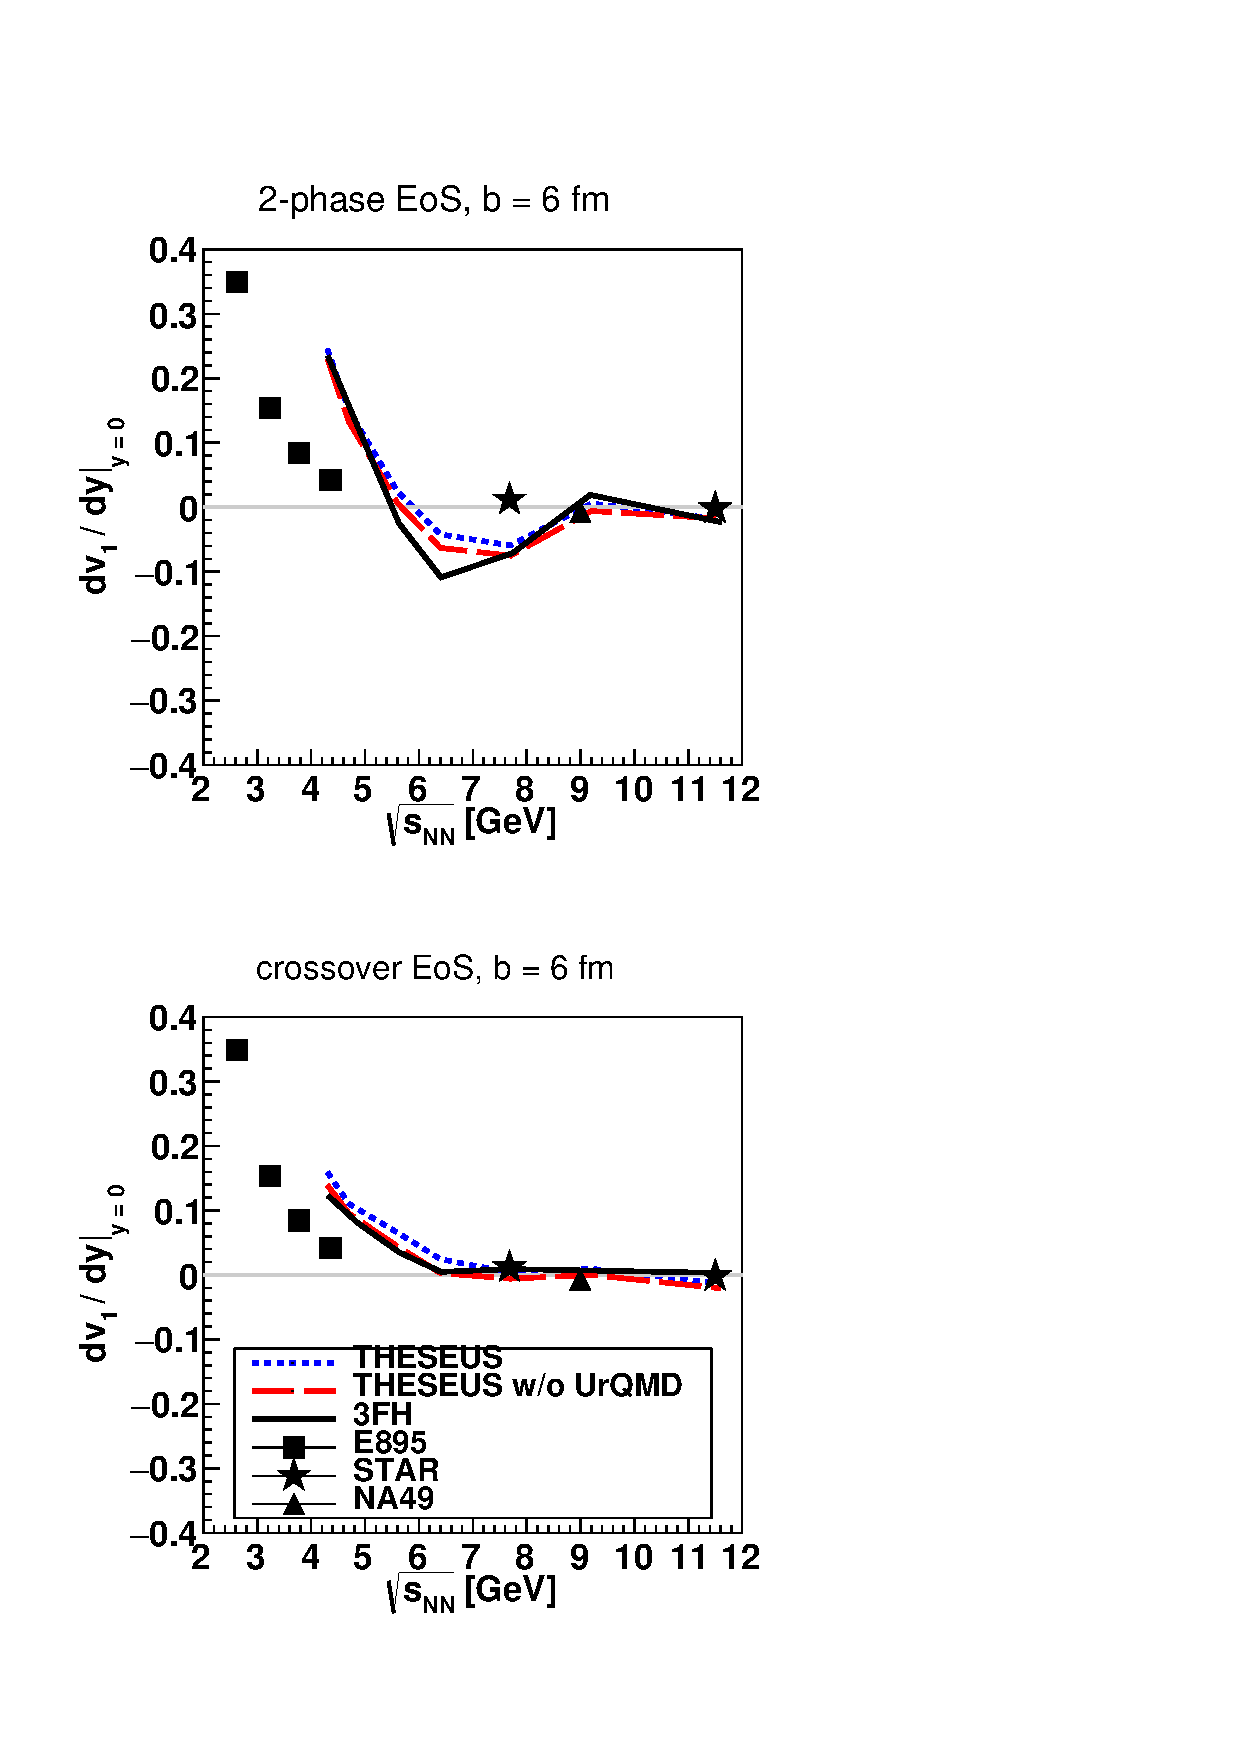
\includegraphics[width=.9\textwidth]{proton_THESEUS_111.pdf}
      \end{figure}  
    \end{block}
    \begin{block}{{\tiny \bf Real PID used:}}
      {\tiny \bf recoTrack->GetPidProbProton() > 0.9}
    \end{block}
    %   {\tiny \bf Real PID used:}
  %  {\tiny recoTrack->GetPidProbProton() > 0.9}   
  \end{columns} 
\end{frame}

\begin{frame}
  \frametitle{\bf \centering Direct flow of light clusters,  $dv_{1} / dy$}
  \begin{columns}[c]
    \column{.35\textwidth}
    \begin{block}{}
      \begin{figure}[H]
        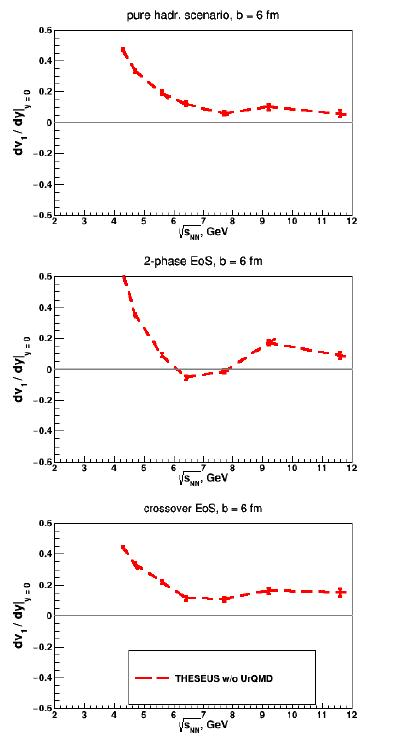
\includegraphics[width=1.0\textwidth]{lightClusters.jpg}
      \end{figure}
    \end{block}
  
    \column{.49\textwidth}
    \begin{block}{}
      \bf
      \begin{itemize}
      \item Light clusters (d, t, h, $\alpha$) can be important indicators for
        the properties of matter produced in HIC at NICA since they probe the
        phase space more locally.

        {\color{red} \item There is an antiflow for $\sqrt{s_{NN}} = 6-7$ GeV only
          for the case of the 2-phase
          EoS while two alternative EoS without a first order phase
          transition do not exhibit the antiflow.}
      %\item
      \end{itemize}
    \end{block}


  \end{columns}
\end{frame}

\begin{frame}[shrink=35]
  \frametitle{{\small Baryon stopping signal for a first-order phase transition}}
  \begin{columns}[c]
    \column{.35\textwidth}
    \begin{block}{}
      \begin{figure}[H]
        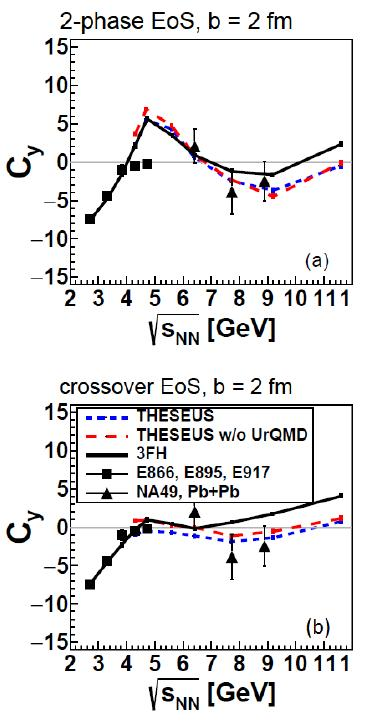
\includegraphics[width=.9\textwidth]{barStopping_curv.jpg}
      \end{figure}
    \end{block}
  
    \column{.49\textwidth}
    \begin{block}{}
     
      $$C_{y} = y_{cm}^{2} \dfrac{d^{3}N_{netProt} / dy^{3}}{dN_{netProt} / dy}$$
        
       $$ C_{y} = \dfrac{y^{2}_{beam} 2a}{c} ~~~ (P_{2}(y) = ay^{2} + by + c) $$
        
       $$ \Delta C_{y} = \dfrac{2 y^{2}_{beam}}{c}\sqrt{(\Delta a)^{2} + \dfrac{a^{2}}{c^{2}} (\Delta c)^{2}}$$
    
    \end{block}
    
    \begin{block}{}
       \begin{figure}[H]
         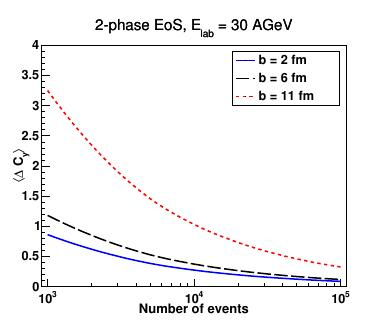
\includegraphics[width=.9\textwidth]{Cy_errorDistrib.jpg}
       \end{figure}
    \end{block}
  \end{columns} 
\end{frame}


\begin{frame}
  \frametitle{{\small Baryon stopping signal for a first-order phase transition}}
  \begin{block}{}
     \begin{figure}[H]
       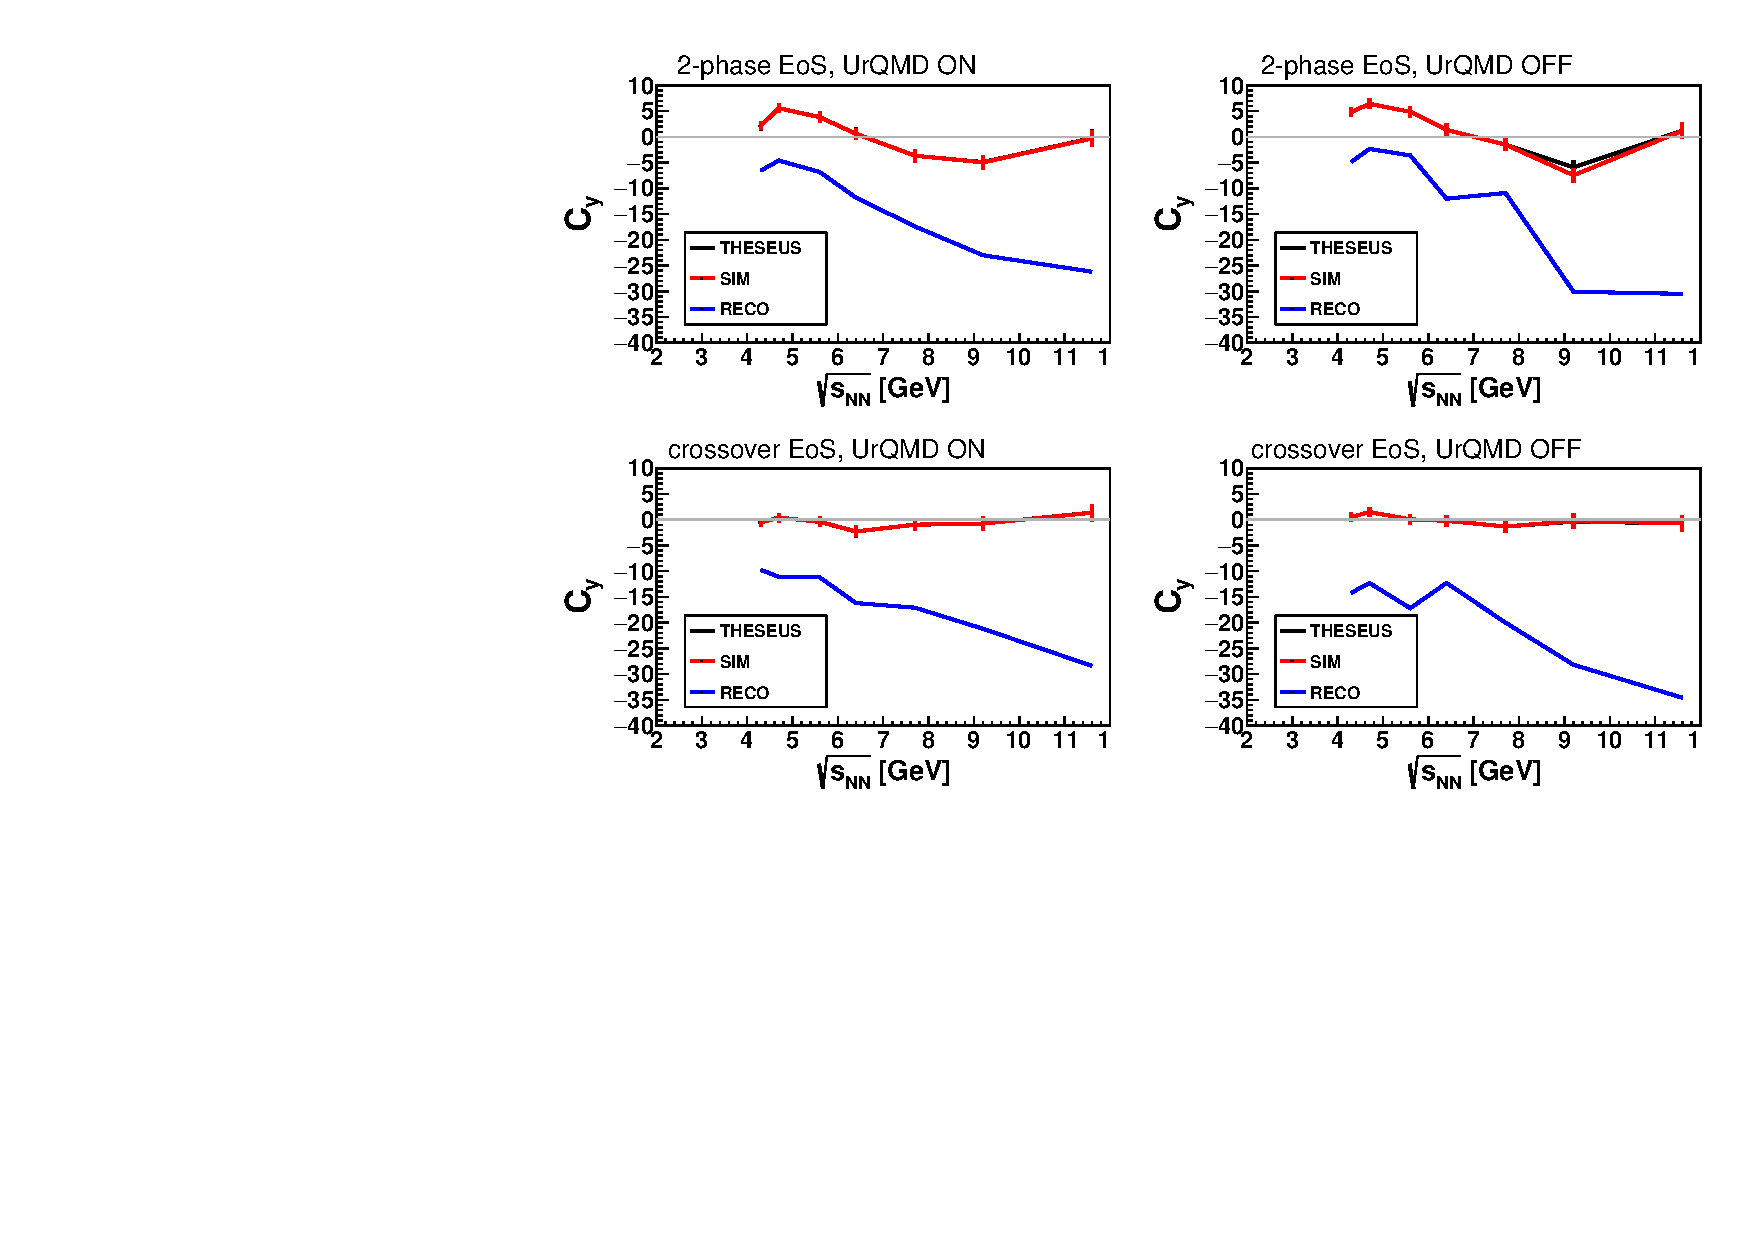
\includegraphics[width=.9\textwidth]{Cy_comparision_noCuts_central.pdf}
     \end{figure}     
  \end{block} 
\end{frame}


\begin{frame}
 
\end{frame}

\begin{frame}
  \frametitle{\bf \centering Do we have "horn"?}
  \begin{columns}[c]
    \column{.33\textwidth}
   \begin{block}{}
     \begin{figure}[H]
       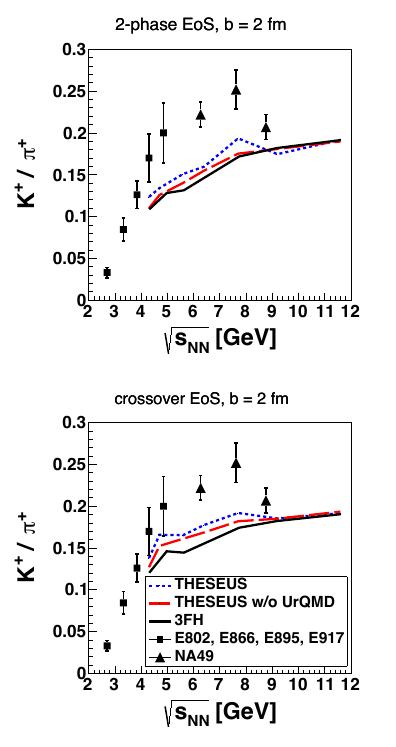
\includegraphics[width=1.\textwidth]{hornPlot.jpg}
     \end{figure}
   \end{block}
   \column{.49\textwidth}
   \begin{block}{}
     \bf
     \begin{itemize}
     \item {\color {blue} As the 3FH-model itself,
       also THESEUS in its present version is not
       yet capable of describing the ”horn” effect discovered in
       the NA49 data for the $K^{+} / \pi^{+}$ ratio.}
     \item {\color {red} No MC-simulations of NICA/MPD w.r.t. to "horn'' done.}
     \end{itemize}
   \end{block}
   \end{columns}
\end{frame}





\begin{frame}
  \bf
  \frametitle{Conclusion}
  \begin{itemize}
  \item Activities concerning creation of a standalone code including {\color {red} 3FH + Particlization + UrQMD-cascade} in a one chain are in progress  
  \item Preliminary results on NICA/MPD MC-simulations showed ...
  \item
  \end{itemize}
  
    

\end{frame}




\end{document} 
